% Working scaffold, 2026-10-20. Not a submission-ready manuscript.
% Original Overleaf ACM sample files are preserved.
\documentclass[sigconf,10pt]{acmart}
\setcopyright{none}
\settopmatter{printacmref=false,printfolios=true}
\renewcommand\footnotetextcopyrightpermission[1]{}
\acmConference[MobiSys 2027 submission draft]{MobiSys 2027 submission draft}{}{}
\acmDOI{}
\acmISBN{}
\usepackage{booktabs}
\usepackage{tabularx}
\newcommand{\todo}[1]{\par\noindent{\color{red!65!black}\textbf{To complete:} #1}\par}
\newcommand{\writingnote}[1]{\par\noindent{\color{blue!55!black}\textbf{Writing plan:} #1}\par}
\newcommand{\figplaceholder}[2]{%
  \fbox{\parbox[c][#1][c]{0.92\linewidth}{\centering\small #2}}}
\title{Policy-Aligned Feature Streaming for Efficient Edge--Cloud VLA Inference}
\author{Author names to be supplied}
\affiliation{\institution{Affiliations to be supplied}\country{Country to be supplied}}
\renewcommand{\shortauthors}{Authors to be supplied}
\begin{document}
\begin{abstract}
\textbf{Working abstract scaffold---not a final research claim.}
Edge--cloud deployment of vision--language--action (VLA) models must
balance communication, edge computation, cloud computation, and control
quality. This paper studies a policy-aligned visual communication interface:
a lightweight edge encoder transmits quantized temporal features, and a
cloud decoder recovers representations for a frozen policy rather than
first reconstructing an image. The design combines student visual
encoding, policy-guided training, and temporal coding without a neural
decoder at the edge. The evaluation is organized around task success,
actual transmitted bytes, end-to-end latency, physical closed-loop
behavior, and deployment boundaries.
\textbf{Pending:} finalize contributions and insert only traceable,
configuration-specific results after fair baselines and physical trials
are complete.
\end{abstract}
\keywords{Vision-language-action models, edge-cloud inference, feature compression, robotic systems}
\maketitle
\begin{center}
\small\textbf{WORKING SCAFFOLD --- 20 OCTOBER 2026}\\
Colored notes and framed figures are planning placeholders, not results.
\end{center}
% Target budget: abstract + introduction, 1.25 pages.
\section{Introduction}
\label{sec:introduction}
\writingnote{Build the argument in five steps: application constraints;
limits of image offloading and conventional splitting; the feature-interface
insight; design challenges; validated contributions and results.}

Edge--cloud VLA inference creates a design choice about the representation
crossing the network boundary. Image compression reduces communication,
but retains image reconstruction and visual encoding at the receiver.
Moving visual computation to the robot changes this tradeoff, but can
overload a resource-constrained edge device. The central question of this
paper is therefore: \emph{what visual representation should a robot
transmit to obtain useful actions promptly without unacceptable loss of
task performance?}

Our working approach makes policy-aligned features the communication
interface. A lightweight student encoder produces compact quantized
representations, temporal prediction reduces redundancy, and a cloud
decoder recovers features consumed by a frozen policy. For the primary
$\pi_{0.5}$ configuration, this replaces the cloud visual encoder and
projection; other backbones may retain additional visual processing.

\paragraph{Challenges.}
Low reconstruction error need not imply correct actions; additional edge
computation can erase communication savings; and temporal coding requires
consistent reference state across devices. Finally, faster inference
does not automatically translate into more successful physical control.

\paragraph{Provisional contributions.}
\begin{enumerate}
  \item A policy-aligned feature communication interface combining compact
  student encoding with action, token, and rate objectives.
  \item A deployable temporal feature stream using quantized references
  and integer entropy coding without a neural decoder at the edge.
  \item An evaluation connecting control quality and actual system cost
  across deployment conditions, with physical closed-loop validation
  explicitly pending.
\end{enumerate}
\todo{Replace provisional contribution wording after mechanism ablations
and physical trials. Do not claim that action-aware compression, DPCM,
rANS, or edge--cloud VLA partitioning is individually new. Insert a compact
result summary only when the associated configurations and raw logs are fixed.}

% Target budget: 1.25 pages.
\section{Background and Motivation}
\label{sec:background}
\subsection{The Observation--Action Loop}
\writingnote{Define observations, camera count, policy requests, action
chunks, and asynchronous execution. Distinguish actuator control rate
from policy invocation rate. Derive an application-specific freshness
or deadline metric instead of assuming that every control step needs
a new VLA inference.}

\subsection{The Cost of Visual Communication}
\label{sec:bg-cost}
\begin{figure}[t]
  \centering
  \figplaceholder{30mm}{PATH COMPARISON PLACEHOLDER\\[4pt]
  Image codec $\rightarrow$ image reconstruction $\rightarrow$ visual tower\\
  Conventional split $\rightarrow$ activation transfer $\rightarrow$ remaining layers\\
  Proposed codec $\rightarrow$ policy-aligned features $\rightarrow$ frozen policy}
  \caption{Planned comparison of visual communication interfaces.
  This is an architectural placeholder, not a performance result.}
  \label{fig:paths}
\end{figure}
\writingnote{Use measured edge, transfer, and cloud costs to motivate the
interface in Figure~\ref{fig:paths}. Separate computation-only and
end-to-end latency. Explain where additional edge work pays off and where
it does not.}

\subsection{Why Policy Alignment Matters}
\label{sec:bg-align}
\writingnote{Contrast pixel quality, teacher-feature similarity, and
closed-loop success. Use matched rate--success curves and controlled
training ablations, not a selected low-rate failure alone.}
\todo{Finalize the RoboCasa input-domain protocol before comparing codecs.
Training-domain AV1 preprocessing is distinct from additional transport
compression. SPARC already uses action-aware training and discusses
latency~\cite{sparc}; the interface and cost distribution are the intended distinction.}

% Target budget: 0.75--1 page.
\section{System Overview}
\label{sec:overview}

\begin{figure*}[t]
  \centering
  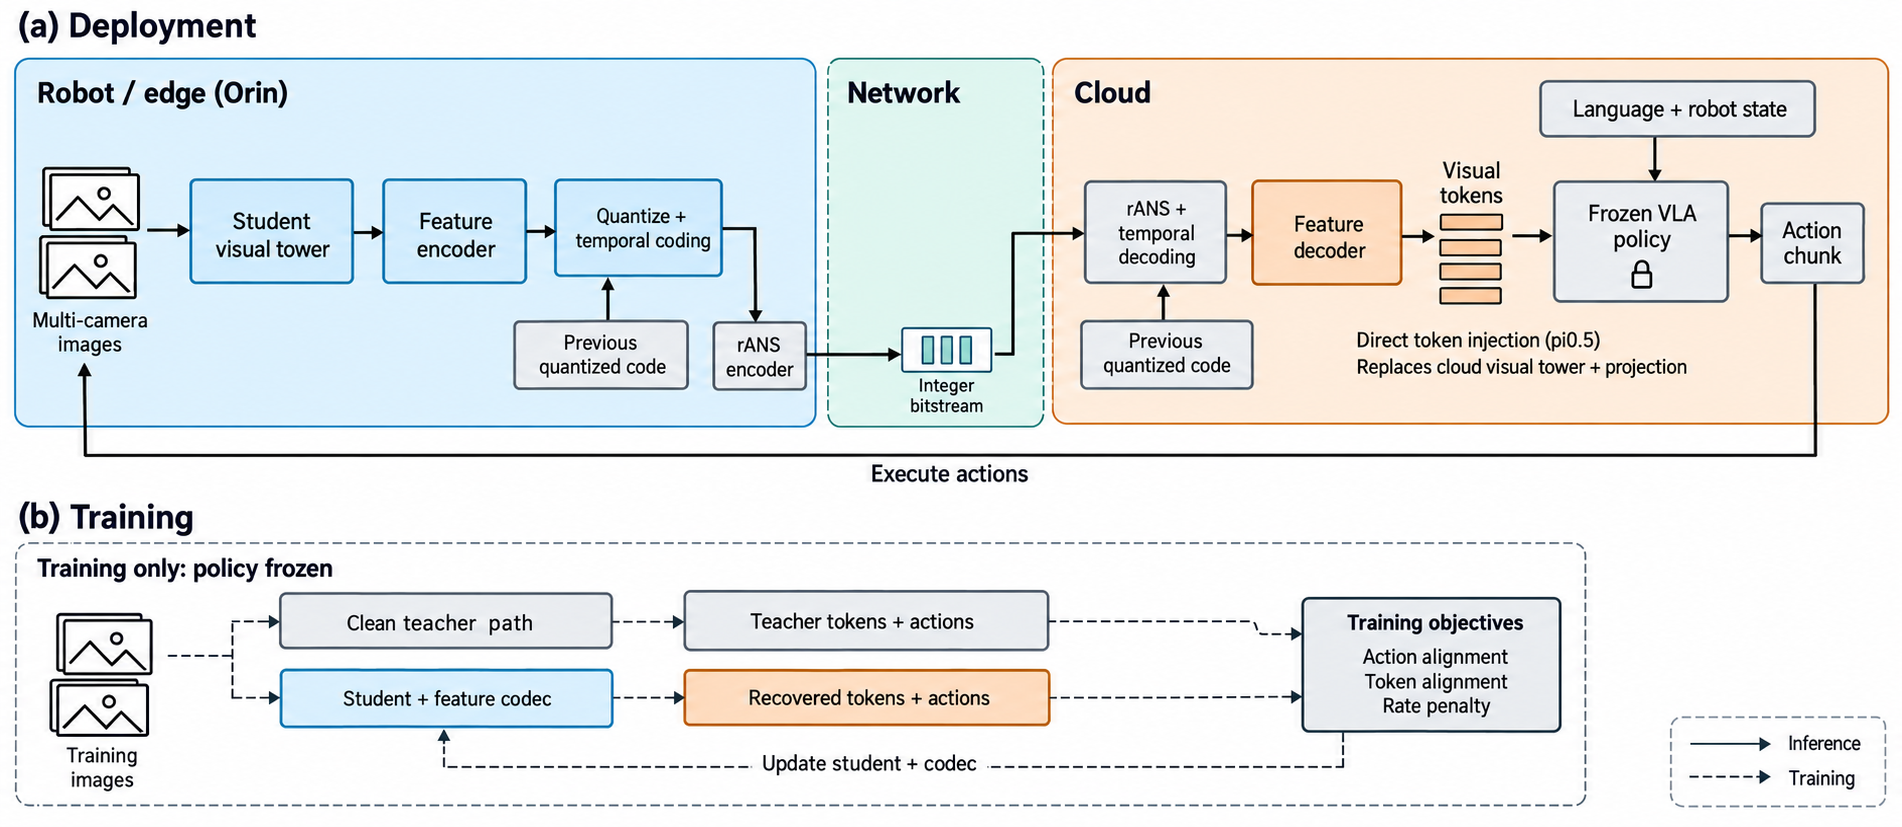
\includegraphics[width=\textwidth]{system-architecture-v1.png}
  \caption{System overview (primary $\pi_{0.5}$ configuration).
  (a) Deployment: the robot turns camera images into an integer bitstream;
  the cloud recovers the policy's visual tokens from the bitstream and runs
  the frozen VLA policy, skipping the cloud visual encoder.
  (b) Training: the student tower and codec are trained against the frozen
  policy's own tokens and actions on clean images, with a rate penalty.}
  \Description{Top panel: on the robot, multi-camera images pass through a
  student visual tower, feature encoder, quantization with temporal coding
  against the previous quantized code, and an rANS encoder; an integer
  bitstream crosses the network; in the cloud, rANS and temporal decoding,
  a feature decoder, and visual tokens feed a frozen VLA policy that also
  receives language and robot state and returns an action chunk. Bottom
  panel: a clean teacher path and the student-plus-codec path produce tokens
  and actions that are compared under action alignment, token alignment,
  and a rate penalty; only the student and codec are updated.}
  \label{fig:overview}
\end{figure*}

Each policy request incurs computation on the robot, transmission over the
network, and computation in the cloud~\cite{neurosurgeon,roboecc}.
Existing designs shift cost among the three (\S\ref{sec:bg-cost}). Image
codecs keep transmission small, but the cloud must still decode each image
and run the policy's visual encoder~\cite{limitnet,sparc}. Splitting the
policy can move that encoder onto the robot~\cite{roboecc}, where it
competes for limited compute. Our system transmits the policy's visual
features instead of images: it spends a small amount of computation on the
robot, sends a compact bitstream, and removes visual encoding from the
cloud, while the policy itself stays unchanged.

\paragraph{Pipeline.}
Figure~\ref{fig:overview}a shows the deployed pipeline. On the robot, a
compact student tower distilled from the policy's visual encoder extracts
features from each camera image, and a feature encoder and quantizer map
them to integer codes. Each code is predicted from the code sent at the
previous upload, except at periodic intra frames, and the residual is
entropy-coded with integer rANS. In the cloud, the receiver reverses the
entropy and temporal coding to recover the codes exactly, and a feature
decoder turns them into visual tokens that replace the output of the
policy's visual encoder. The frozen policy consumes these tokens together
with the language instruction and robot state, which bypass the codec, and
returns an action chunk.

The design must solve four problems.

\paragraph{Preserving actions rather than appearance.}
Faithful reconstruction of images or features does not guarantee that the
policy acts the same (\S\ref{sec:bg-align}). We therefore supervise the
student tower and codec with the frozen policy's own outputs on clean
images. An action term matches the actions produced from recovered tokens
to those produced from clean images, a token term matches the tokens
themselves, and a rate term bounds the bitstream size
(Figure~\ref{fig:overview}b, \S\ref{sec:design-objective}).

\paragraph{Keeping robot computation small.}
Running the policy's visual encoder at every upload adds substantial
latency on resource-constrained robot hardware. The robot instead runs the
distilled student tower, trained jointly with the codec, so its work is
limited to the student tower, the feature encoder, and entropy coding
(\S\ref{sec:design-objective}).

\paragraph{Temporal coding without a decoder on the robot.}
Video codecs predict each frame from a reconstructed reference, so the
encoder also runs the decoder. For a learned codec, this would place a
neural decoder on the robot, and floating-point differences between the
robot and the cloud could desynchronize the reference. We instead predict
in the space of quantized codes, which both ends hold exactly, and use
integer-only rANS so that ARM and x86 hosts produce identical bitstreams
(\S\ref{sec:design-temporal}).

\paragraph{Fitting backbones with different visual interfaces.}
Backbones consume visual features in different forms: $\pi_{0.5}$ takes
projected SigLIP tokens, whereas OpenVLA-OFT fuses features from two
visual towers. The pipeline structure is shared; the student tower and
feature decoder are adapted to each backbone's interface, and the codec is
trained once per backbone (\S\ref{sec:design-integration}).

% Target budget: 2.50 pages.
\section{Design}
\label{sec:design}
\subsection{Policy-Aligned Compact Features}
\label{sec:design-objective}
\writingnote{Define the teacher, student tower, feature bottleneck,
quantizer, and cloud decoder with explicit tensor shapes. Introduce the
primary $\pi_{0.5}$ configuration before backbone-specific differences.}

The working training objective combines action alignment, teacher-token
matching, and a rate penalty:
\begin{equation}
  \mathcal{L} =
  \lambda_a \mathcal{L}_{\mathrm{action}}+
  \lambda_t \mathcal{L}_{\mathrm{token}}+
  \lambda_r \mathcal{L}_{\mathrm{rate}}.
  \label{eq:objective}
\end{equation}
\todo{Match Equation~\ref{eq:objective} to the training code, including
normalization, loss weights, rate controller, and quantization estimator.
Clean-policy outputs are the action target; do not describe them as human
expert labels. Define the backbone-specific action objective precisely.}

\subsection{Decoder-Free Temporal Coding at the Edge}
\label{sec:design-temporal}
\writingnote{Define the quantized code, reference, residual, intra frame,
and GOP mathematically. Explain why the reference does not require a
neural reconstruction decoder at the edge. Distinguish exact integer
coding from floating-point model execution.}

\paragraph{Bitstream and synchronization.}
\todo{Specify rANS state, frequency tables, payload headers, camera and
session identifiers, reference initialization, and reset rules. Include
cross-device round-trip tests. Quantized-code losslessness does not imply
identical neural outputs on all devices.}

\paragraph{Temporal training.}
\writingnote{Explain how training rolls out intra/inter-frame states in
the same way as deployment. Evaluate GOP and motion sensitivity, especially
for wrist cameras. State whether dropped or reordered messages can occur
under the chosen transport.}

\subsection{Integration with Frozen VLA Backbones}
\label{sec:design-integration}
\begin{table}[t]
  \caption{Backbone adaptation map from the handoff notes; verify exact
  interfaces against the implementation before submission.}
  \label{tab:interfaces}
  \centering\small
  \begin{tabularx}{\columnwidth}{lX}
    \toprule
    Backbone & Feature interface and scope \\
    \midrule
    $\pi_{0.5}$ & Replace cloud SigLIP and projection with recovered policy tokens. \\
    OpenVLA-OFT & Adapt to the dual-tower visual representation; use policy-matched training. \\
    \bottomrule
  \end{tabularx}
\end{table}
\writingnote{Explain what is shared across Table~\ref{tab:interfaces}
and what is retrained. Do not present model splitting alone as a novel
mechanism.}

% Target budget: 0.75 pages.
\section{Implementation}
\label{sec:implementation}
\subsection{Runtime and Deployment}
\writingnote{Record Orin model and power mode, cloud GPU, software versions,
precision, compilation, warm-up, camera resolution/count, asynchronous
LeRobot integration, and the feature injection interface. Explain any
changes to baseline implementations.}

\subsection{Measurement and Reproducibility}
\writingnote{Define timestamps for observation capture, encoding, send,
receive, decoding, policy completion, and action application. Document
clock synchronization. Report actual payload and application/network
overhead separately; define KB versus KiB.}

\todo{Create a run manifest containing policy and codec checkpoint IDs,
code revision, training configuration, hardware, seeds, input-domain
protocol, raw log paths, and metric script version. Preserve original
logs rather than relying on summary tables alone.}

% Target budget: 4.25 pages. Questions, not fabricated results.
\section{Evaluation}
\label{sec:evaluation}
\subsection{Setup, Baselines, and Statistical Protocol}
\writingnote{Introduce datasets/tasks, physical setup, hardware, network
conditions, and baselines: reference input, JPEG, tuned low-latency H.264,
policy-matched SPARC, and a feasible conventional feature-transfer baseline.
Use matched hardware, precision, training budgets, and evaluation windows.}
\todo{Define primary endpoints before new trials. Report paired success
differences and confidence intervals when pairing is valid. Nonsignificance
is not equivalence; any existing post-hoc noninferiority margin must be
identified as post hoc.}

\subsection{Control Quality versus Communication Cost}
\begin{figure}[t]
  \centering
  \figplaceholder{28mm}{RATE--SUCCESS CURVES PLACEHOLDER\\[4pt]
  Panel A: LIBERO\\Panel B: RoboCasa\\
  Actual bytes per upload; success rates with uncertainty\\
  Multiple rate points for each relevant method}
  \caption{Planned rate--control-quality comparison. No curves have been
  fabricated; populate from traceable completed runs.}
  \label{fig:rate-success}
\end{figure}
\writingnote{Lead with the primary $\pi_{0.5}$ configuration. Distinguish
the full success-rate sample from the subset used to measure actual rANS
payload. Explain the RoboCasa preprocessing protocol before interpreting
low-rate failures.}

\begin{table}[t]
  \caption{Main-result schema. All cells below are intentionally pending;
  rows must refer to a consistent evaluation protocol.}
  \label{tab:main-results}
  \centering\small
  \begin{tabularx}{\columnwidth}{lXXX}
    \toprule
    Method & Episodes & Success / difference CI & Actual bytes \\
    \midrule
    Reference & TBD & TBD & TBD \\
    JPEG & TBD & TBD & TBD \\
    H.264 & TBD & TBD & TBD \\
    SPARC & TBD & TBD & TBD \\
    Ours & TBD & TBD & TBD \\
    \bottomrule
  \end{tabularx}
\end{table}
\todo{Do not infer a significant ours-versus-H.264 difference because
only one method differs significantly from the reference. Use the direct
comparison. Separate sample denominators and input protocols.}

\subsection{Deployed Latency and Physical Closed-Loop Behavior}
\begin{figure}[t]
  \centering
  \figplaceholder{27mm}{SYSTEM LATENCY PLACEHOLDER\\[4pt]
  End-to-end CDF / p50 / p95 under one deployment\\
  Consistently measured edge, transport, and cloud stages\\
  Label device replay separately from physical trials}
  \caption{Planned actual-system latency evaluation. Stage medians are
  not necessarily additive.}
  \label{fig:latency}
\end{figure}

\begin{figure}[t]
  \centering
  \figplaceholder{27mm}{PHYSICAL CLOSED-LOOP RESULTS --- PENDING\\[4pt]
  Task success and completion time\\
  Observation age / action starvation / deadline misses\\
  Normal and representative constrained network conditions}
  \caption{Planned physical validation linking system timing to control
  outcomes. Replay uploads are not independent physical task trials.}
  \label{fig:physical}
\end{figure}
\writingnote{Use randomized method blocks and standardized task resets.
Collect success and timing for the same trials. Size the final experiment
from a meaningful effect or tolerance and pilot data; twenty trials per
arm do not automatically establish a narrow noninferiority margin.}

\subsection{Deployment Boundaries and Network Sensitivity}
\begin{figure}[t]
  \centering
  \figplaceholder{25mm}{OPERATING-REGION PLACEHOLDER\\[4pt]
  Bandwidth / RTT / jitter / cloud compute\\
  Real measurements first; analytical predictions labeled\\
  Include conditions where gains shrink or reverse}
  \caption{Planned sensitivity study. Analytical queueing results must
  not be presented as measured multi-robot deployments.}
  \label{fig:boundaries}
\end{figure}
\todo{Measure sustained operation, thermal behavior, and reference-state
recovery under supported network failures. Use representative traces
and record the shaping configuration.}

\subsection{Generality across VLA Backbones}
\writingnote{Report OFT with policy-matched codecs and baselines.
Separate feasibility from fully controlled comparison. Identify measured
versus estimated bitrates and training costs.}
\todo{Complete contemporaneous OFT runs and dedicated SPARC evaluation.
Do not compare a 400-episode arm to a 200-episode transferred-checkpoint
arm as though both were a matched primary experiment.}

\subsection{Ablations and Resource Costs}
\begin{figure}[t]
  \centering
  \figplaceholder{25mm}{MATCHED ABLATIONS PLACEHOLDER\\[4pt]
  Without action loss; without temporal prediction\\
  Student versus teacher visual tower\\
  Quality, actual bytes, latency, and memory together}
  \caption{Planned mechanism analysis. Fix training data, budgets, and
  evaluation protocol; disclose unavoidable rate differences.}
  \label{fig:ablations}
\end{figure}

\begin{table}[t]
  \caption{Resource-reporting schema. Power mode is not measured energy.}
  \label{tab:resources}
  \centering\small
  \begin{tabularx}{\columnwidth}{lX}
    \toprule
    Metric & Required measurement \\
    \midrule
    Edge / cloud latency & Full path and component boundaries \\
    Peak memory & Matched precision and batching \\
    Energy & Joules per request and per successful task \\
    Training cost & Hardware, time, data, per-policy retraining \\
    Streaming overhead & Headers, state, initialization, recovery \\
    \bottomrule
  \end{tabularx}
\end{table}

% Target budget: 0.50 pages.
\section{Discussion and Limitations}
\label{sec:limitations}
\writingnote{Discuss distribution shift, per-policy retraining, edge
compute requirements, retained cloud computation in some backbones,
temporal reference assumptions, and deployment-dependent latency gains.}
\todo{Retain the LIBERO-Plus degradation and the unfavorable Lego offline
action-deviation result with their exact scope. Do not imply that all
physical tasks or all perturbations benefit. Explain why the modest
observed $\pi_{0.5}$ throughput gain does not support a large scalability claim.}

% Target budget: 0.50 pages.
\section{Related Work}
\label{sec:related}
\paragraph{Task-aware visual communication.}
LimitNet studies progressive content-aware image offloading under severe
device and network constraints~\cite{limitnet}. SPARC addresses learned
image compression for VLA models with action-aware training~\cite{sparc}.
\writingnote{Explain the image-reconstruction versus policy-feature
interface distinction without claiming that task-aware compression is new.}

\paragraph{Edge--cloud VLA inference.}
RoboECC and RAPID study collaborative VLA deployment and partitioned
inference~\cite{roboecc,rapid}.
\writingnote{Compare the representation and training mechanisms, not
only the location of a model split.}

\paragraph{Timely mobile and robotic inference.}
ARIA and TimelyLLM motivate application-sensitive evaluation of inference
systems~\cite{aria,timelyllm}.
\writingnote{Position this work as a visual communication system, not a
new general scheduler. Replace the temporary source list with verified
full bibliographic metadata before submission.}

% Target budget: 0.25 pages.
\section{Conclusion}
\label{sec:conclusion}
\writingnote{Answer the representation-interface question, summarize the
validated quality--cost tradeoff, and state its operating conditions.
Do not introduce new experiments or stronger claims than the evaluation.}
\todo{Write the final conclusion after the physical experiments and fair
baseline comparisons are complete.}

% Temporary source list, NOT camera-ready bibliographic metadata.
% Titles and URLs are supplied instead of inventing author lists or dates.
\begin{thebibliography}{6}
\bibitem{limitnet}
\emph{LimitNet: Progressive, Content-Aware Image Offloading for Extremely
Weak Devices \& Networks}. MobiSys 2024.
\url{https://arxiv.org/abs/2504.13736}.
\bibitem{aria}
\emph{ARIA: Optimizing Vision Foundation Model Inference on Heterogeneous
Mobile Processors for Augmented Reality}. MobiSys 2025.
\url{https://lovelyzzkei.github.io/assets/pdf/mobisys25-aria.pdf}.
\bibitem{timelyllm}
\emph{TimelyLLM: Time-sensitive LLM Serving System for Physical-I/O
Limited Agents}. MobiSys 2026.
\url{https://www.anuragkhandelwal.com/papers/timelyllm/}.
\bibitem{sparc}
\emph{Learned Image Compression for Vision-Language-Action Models}.
arXiv:2606.16253, version 2.
\url{https://arxiv.org/abs/2606.16253}.
\bibitem{roboecc}
\emph{RoboECC: Multi-Factor-Aware Edge-Cloud Collaborative Deployment
for VLA Models}. arXiv:2603.20711.
\url{https://arxiv.org/abs/2603.20711}.
\bibitem{rapid}
\emph{RAPID: Redundancy-Aware and Compatibility-Optimal Edge-Cloud
Partitioned Inference for Diverse VLA Models}. arXiv:2603.07949.
\url{https://arxiv.org/abs/2603.07949}.
\bibitem{neurosurgeon}
Y. Kang, J. Hauswald, C. Gao, A. Rovinski, T. Mudge, J. Mars, and L. Tang.
\emph{Neurosurgeon: Collaborative Intelligence Between the Cloud and Mobile
Edge}. ASPLOS 2017. doi:10.1145/3037697.3037698.
\end{thebibliography}

\appendix
\section{Reproducibility Checklist}
\label{app:reproducibility}
\writingnote{Include run manifests, checkpoint hashes, dependency versions,
training settings, preprocessing, randomization and reset protocols,
bitstream validation, and metric-generation commands. Essential fairness
information must remain in the main paper.}

\section{Additional Results and Diagnostics}
\writingnote{Include full task breakdowns, secondary rate points,
input-domain diagnostics, additional negative results, and explicitly
labeled analytical models. Keep historical versions separate.}

\section{Draft Status and Writing Assistance}
This document is an AI-assisted working scaffold assembled from the
project's handoff notes and research outline. Colored writing notes,
placeholder figures, author placeholders, and the temporary reference
list must be reviewed before submission. No new experiment is reported
as completed by this scaffold.
\todo{Apply the conference's current disclosure requirements to any
generated text retained in the submitted paper. Verify all bibliographic
metadata and author information.}

\end{document}
